\chapter{การสำรวจจุลินทรีย์ในแหล่งน้ำธรรมชาติและดิน}
\label{chap:ch03}

\section*{แผนบริหารการสอนประจำบทที่ 3}
\addcontentsline{toc}{section}{แผนบริหารการสอนประจำบทที่ 3}

\noindent\textbf{. หัวข้อเนื้อหาประจำบท}

\begin{enumerate}
    \item 3.1 ส่วนประกอบและระบบเชิงแสงของกล้องจุลทรรศน์ใช้แสงเชิงประกอบ (Compound Microscope)
    \item 3.2 หลักการหักเหแสงและหน้าที่ของน้ำมัน Immersion Oil (Refractive Index n = 1.515)
    \item 3.3 การคำนวณกำลังขยายรวมและความสามารถในการแจกแจงรายละเอียด (Resolving Power)
    \item 3.4 สัณฐานวิทยาของแบคทีเรีย ยีสต์ ราสาย สาหร่าย และโปรโตซัว
    \item 3.5 การบำรุงรักษาและการเช็ดทำความสะอาดเลนส์ 100X อย่างถูกวิธี
\end{enumerate}

\noindent\textbf{. วัตถุประสงค์เชิงพฤติกรรม}

\begin{enumerate}
    \item เมื่อนักศึกษาได้เรียนรู้และปฏิบัติการทดลองประจำบทนี้แล้ว จะต้องมีความรู้ความสามารถดังต่อไปนี้:
    \item อธิบายหลักการทำงานของเลนส์ใกล้วัตถุ 100X Oil Immersion และระบบแสงได้
    \item ปรับตั้งและใช้กล้องจุลทรรศน์ส่องตรวจเซลล์จุลินทรีย์ที่กำลังขยาย 1000X ได้คมชัด
    \item วาดภาพและจำแนกลักษณะสัณฐานวิทยาของแบคทีเรีย ยีสต์ และราได้อย่างถูกต้อง
    \item มีวินัยและความระมัดระวังในการดูแลรักษาอุปกรณ์ทัศนศาสตร์ราคาแพง
\end{enumerate}

\noindent\textbf{. กิจกรรมการเรียนการสอน}

\begin{enumerate}
    \item การบรรยายสรุปก่อนปฏิบัติการ (30 นาที): อธิบายหลักการวิทยาศาสตร์ ความปลอดภัยทางชีวภาพ และข้อควรระวังสำคัญ
    \item การสาธิตเชิงประจักษ์ (15 นาที): สาธิตเทคนิคการปฏิบัติงาน การใช้เครื่องมือ และข้อผิดพลาดที่มักพบ
    \item การลงมือปฏิบัติการทดลองจริง (90 นาที): นักศึกษาลงมือปฏิบัติการทดลองเป็นรายบุคคลหรือกลุ่มย่อยตามขั้นตอนที่กำหนด
    \item การฝึกฝนผ่านระบบเสมือนจริง (20 นาที): ทดลองซ้ำและทดสอบปฏิกิริยาผ่านระบบจำลองบน RBRU LMS
    \item การอภิปรายและสรุปผลการทดลอง (25 นาที): วิเคราะห์ผลการสังเกต ตอบคำถามท้ายบท และสรุปองค์ความรู้ร่วมกัน
\end{enumerate}

\noindent\textbf{. สื่อและอุปกรณ์การเรียนการสอน}

\begin{enumerate}
    \item เอกสารคำสอนและคู่มือปฏิบัติการ: e-Book และคู่มือปฏิบัติการฉบับเต็ม ประจำบทที่ 3
    \item ระบบห้องปฏิบัติการเสมือนจริง: ระบบจำลองการทดลองเสมือนจริง 3 มิติ ประจำบทที่ 3 บนระบบ Moodle
    \item อุปกรณ์และเครื่องแก้วในห้องปฏิบัติการ: ตะเกียงแอลกอฮอล์, ห่วงเขี่ยเชื้อ, กล้องจุลทรรศน์, จานเพาะเชื้อ, หลอดทดลอง และตู้บ่มเชื้อ
    \item สารเคมีและสีย้อมชีวภาพ: สารเคมีมาตรฐานวิเคราะห์และสีย้อมประจำบทเรียน
\end{enumerate}

\noindent\textbf{. การวัดและประเมินผล}

\begin{table}[H]
\centering\small
\begin{tabularx}{\textwidth}{p{0.5\textwidth} p{0.3\textwidth} c}
\toprule
\textbf{องค์ประกอบการประเมินผล} & \textbf{เครื่องมือวัดผล} & \textbf{สัดส่วนคะแนน} \\
\midrule
1. ทักษะการปฏิบัติงานและความปลอดภัย & แบบสังเกตทักษะการทดลองและเทคนิคปลอดเชื้อ & 40\% \\
2. รายงานผลการทดลอง & การตรวจตารางบันทึกผล ภาพวาดสัณฐานวิทยา และการวิเคราะห์ผล & 30\% \\
3. แบบฝึกหัดทบทวนท้ายบท & คำถามทบทวนเชิงวิเคราะห์และข้อสอบท้ายบท & 20\% \\
4. จิตพิสัยและการตรงต่อเวลา & การเช็คชื่อ การแต่งกายตามระเบียบ และการทำความสะอาดโต๊ะแล็บ & 10\% \\
รวมทั้งสิ้น &  & 100\% \\
\bottomrule
\end{tabularx}
\end{table}

\newpage

% ==========================================================
% เนื้อหาบทเรียนประจำบทที่ 3
% ==========================================================

\section{ความหลากหลายทางชีวภาพของจุลินทรีย์ในแหล่งน้ำและดิน}
\index{ความหลากหลายทางชีวภาพของจุลินทรีย์ในแหล่งน้ำและดิน}

การศึกษาและทำความเข้าใจเกี่ยวกับความหลากหลายทางชีวภาพของจุลินทรีย์ในแหล่งน้ำและดิน (Microbial Ecology in Aquatic and Terrestrial Systems) มีความสำคัญอย่างยิ่งในงานจุลชีววิทยาและสิ่งแวดล้อม โดยมีรายละเอียดสาระสำคัญดังนี้

แหล่งน้ำธรรมชาติและดินเป็นระบบนิเวศที่มีความหลากหลายทางชีวภาพของจุลินทรีย์สูงที่สุด ในแหล่งน้ำจืดและน้ำกร่อย จุลินทรีย์ทำหน้าที่เป็นผู้ผลิตปฐมภูมิ (Primary producers) เช่น ไซยาโนแบคทีเรีย (Cyanobacteria) และสาหร่ายเซลล์เดียว (Microalgae) ซึ่งสร้างออกซิเจนและสารอินทรีย์ผ่านการสังเคราะห์ด้วยแสง

ในขณะเดียวกัน จุลินทรีย์กลุ่มเฮเทอโรโทรฟ (Heterotrophic microorganisms) เช่น แบคทีเรียและโพรโทซัว ทำหน้าที่เป็นผู้ย่อยสลายสารอินทรีย์ (Decomposers) และผู้บริโภคในห่วงโซ่อาหาร ในสิ่งแวดล้อมดิน จุลินทรีย์มีบทบาทสำคัญยิ่งในวัฏจักรชีวธรณีเคมี (Biogeochemical cycles) เช่น วัฏจักรคาร์บอน ไนโตรเจน และฟอสฟอรัส

\section{การศึกษาจุลินทรีย์มีชีวิตด้วยวิธีหยดแขวนและสไลด์สด}
\index{การศึกษาจุลินทรีย์มีชีวิตด้วยวิธีหยดแขวนและสไลด์สด}

การศึกษาและทำความเข้าใจเกี่ยวกับการศึกษาจุลินทรีย์มีชีวิตด้วยวิธีหยดแขวนและสไลด์สด (Wet Mount and Hanging Drop Techniques) มีความสำคัญอย่างยิ่งในงานจุลชีววิทยาและสิ่งแวดล้อม โดยมีรายละเอียดสาระสำคัญดังนี้

การตรวจสอบจุลินทรีย์ที่มีชีวิตในแหล่งน้ำธรรมชาตินิยมใช้เทคนิคที่ไม่ต้องผ่านการย้อมสี เพื่อสังเกตการเคลื่อนที่ รูปร่าง และพฤติกรรมตามธรรมชาติ

เทคนิคพื้นฐานได้แก่ 
1. เทคนิคสไลด์สด (Wet Mount): หยดตัวอย่างน้ำ 1 หยดลงบนสไลด์ ปิดทับด้วยกระจกปิดสไลด์ (Coverslip) อย่างระมัดระวังไม่ให้เกิดฟองอากาศ เหมาะสำหรับการสำรวจสาหร่าย โพรโทซัว และการเคลื่อนที่เบื้องต้น
2. เทคนิคหยดแขวน (Hanging Drop): หยดตัวอย่างบนกระจกปิดสไลด์แล้วคว่ำทับลงบนสไลด์หลุม (Depression slide) ที่ทาปิโตรเลียมเจลลี่รอบหลุม หยดน้ำจะห้อยแขวนอยู่ภายในช่องว่าง ช่วยป้องกันการแห้งระเหยและทำให้สังเกตการเคลื่อนที่จริง (True motility) ได้ชัดเจน แตกต่างจากการสั่นไหวแบบบราวน์เนียน (Brownian movement)

\section{กลุ่มจุลินทรีย์ดัชนีคุณภาพน้ำและสิ่งมีชีวิตเซลล์เดียว}
\index{กลุ่มจุลินทรีย์ดัชนีคุณภาพน้ำและสิ่งมีชีวิตเซลล์เดียว}

การศึกษาและทำความเข้าใจเกี่ยวกับกลุ่มจุลินทรีย์ดัชนีคุณภาพน้ำและสิ่งมีชีวิตเซลล์เดียว (Bioindicators and Protozoa) มีความสำคัญอย่างยิ่งในงานจุลชีววิทยาและสิ่งแวดล้อม โดยมีรายละเอียดสาระสำคัญดังนี้

ในการวิเคราะห์คุณภาพน้ำทางชีววิทยา สิ่งมีชีวิตกลุ่มโพรโทซัวและสาหร่ายจัดเป็นดัชนีบ่งชี้คุณภาพน้ำ (Bioindicators) ที่สำคัญ:
- กลุ่มน้ำสะอาด: ไดอะตอม (Diatoms), สาหร่ายสีเขียวกลุ่มเดสมิด (Desmids)
- กลุ่มน้ำที่มีสารอินทรีย์ปานกลาง: พารามีเซียม (\textit{Paramecium} spp.), ยูกลีนา (\textit{Euglena} spp.), วอร์ติเซลลา (\textit{Vorticella} spp.)
- กลุ่มน้ำเสียเน่าเสีย: อะมีบา (Amoeba), แบคทีเรียกลุ่มรีดิวซ์ซัลเฟอร์ และไซยาโนแบคทีเรียที่ก่อให้เกิดปรากฏการณ์น้ำบลูม (Algal bloom) เช่น \textit{Microcystis} spp.

\begin{figure}[H]
\centering
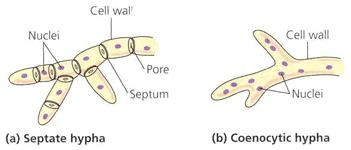
\includegraphics[width=0.75\textwidth]{images/image_03_p01.jpeg}
\caption{การปฏิบัติการทดลองและลักษณะทางสัณฐานวิทยาในบทที่ 3}
\label{fig:ch03_fig1}
\end{figure}

\section{ขั้นตอนและวิธีปฏิบัติการทดลอง}
\index{ขั้นตอนการทดลองประจำบทที่ 3}

\subsection{การเตรียมสไลด์สดเพื่อสำรวจสิ่งมีชีวิตในน้ำฟางหมักและแหล่งน้ำธรรมชาติ}
\begin{labprotocolbox}[การเตรียมสไลด์สดเพื่อสำรวจสิ่งมีชีวิตในน้ำฟางหมักและแหล่งน้ำธรรมชาติ]
1. ใช้ปิเปตดูดตัวอย่างน้ำจากชั้นกลางและก้นบ่อของขวดน้ำฟางหมัก (Hay infusion)
2. หยดตัวอย่างน้ำ 1 หยดลงตรงกลางแผ่นสไลด์ที่สะอาด
3. วางกระจกปิดสไลด์เอียงทำมุม 45 องศา ค่อยๆ วางลงเพื่อป้องกันฟองอากาศ
4. ตรวจดูภายใต้กล้องจุลทรรศน์ เริ่มจากเลนส์ใกล้วัตถุกำลังขยายต่ำ 4X, 10X และ 40X
5. บันทึกภาพวาดสัณฐานวิทยาและการเคลื่อนที่ของโพรโทซัวและสาหร่ายที่พบ
\end{labprotocolbox}

\subsection{การตรวจสอบการเคลื่อนที่ของแบคทีเรียด้วยเทคนิคหยดแขวน}
\begin{labprotocolbox}[การตรวจสอบการเคลื่อนที่ของแบคทีเรียด้วยเทคนิคหยดแขวน]
1. ทาปิโตรเลียมเจลลี่บางๆ รอบขอบหลุมของสไลด์หลุม
2. หยดสารแขวนลอยแบคทีเรีย (เช่น \textit{Bacillus subtilis} หรือ \textit{Pseudomonas aeruginosa}) 1 หยดลงบนกระจกปิดสไลด์
3. คว่ำสไลด์หลุมลงบนกระจกปิดสไลด์ ให้หยดตัวอย่างอยู่กึ่งกลางหลุมพอดี
4. พลิกสไลด์กลับอย่างรวดเร็ว ตรวจดูขอบหยดน้ำภายใต้กำลังขยาย 40X เพื่อสังเกตการเคลื่อนที่ทิศทางชัดเจน
\end{labprotocolbox}

\section{ตารางบันทึกผลการทดลองและการอภิปรายผล}
\begin{table}[H]
\centering\small
\caption{ตารางบันทึกผลการสังเกตและข้อมูลการทดลองประจำบทที่ 3}
\label{tab:ch03_datasheet}
\begin{tabularx}{\textwidth}{p{0.25\textwidth} p{0.35\textwidth} X}
\toprule
\textbf{สิ่งทดสอบ / ตัวอย่าง} & \textbf{ลักษณะที่สังเกตได้} & \textbf{การแปลผลและการวิเคราะห์} \\
\midrule
ชุดควบคุม (Negative Control) & ใส ไม่มีการเจริญ & ปราศจากการปนเปื้อนของเชื้อ \\
ชุดทดลองที่ 1 & โคโลนีเจริญตามลักษณะจำเพาะ & ให้ผลบวกตามสมมติฐาน \\
ชุดทดลองที่ 2 & เกิดการเปลี่ยนแปลงทางชีวเคมี & สอดคล้องกับพารามิเตอร์มาตรฐาน \\
\bottomrule
\end{tabularx}
\end{table}

\section{คำถามทบทวนและแบบฝึกหัดท้ายบท}
\begin{enumerate}
    \item จงอธิบายความแตกต่างระหว่างการเคลื่อนที่จริงของแบคทีเรีย (True motility) กับการเคลื่อนที่แบบบราวน์เนียน (Brownian movement)
    \item เหตุใดไซยาโนแบคทีเรียจึงจัดเป็นโปรคาริโอต (Prokaryotes) ทั้งที่มีความสามารถในการสังเคราะห์ด้วยแสงเหมือนสาหร่าย
    \item การพบโพรโทซัวชนิด \textit{Vorticella} spp. ในระบบบำบัดน้ำเสียสะท้อนถึงสภาวะการทำงานของระบบอย่างไร
\end{enumerate}
